\section{Реализация библиотеки алгоритмов для полулокальных задач}\label{librarySection}
Как было отмечено в обзоре полулокальных задач,
существует необходимость в реализации большей части алгоритмов.
% В данном разделе будет описана реализация и архитектура библиотеки алгоритмов, связанных с полулокальными задачами.

% В качестве языка программирования был выбран \emph{Kotlin}

\subsection{Архитектура библиотеки}
В качестве языка программирования для написания библиотеки\footnote{https://github.com/NikitaMishin/SemiLocalLcs, дата обращения 26.05.2020} был выбран язык \emph{Kotlin}.


Код библиотеки можно  разделить на два логических модуля:
\begin{itemize}
    \item модуль \emph{semilocalProblem}  (рис.~\ref{fig:libraryProblem});
    \item модуль \emph{semilocalApplication} (рис.~\ref{fig:libraryApplication}).
\end{itemize}



\subsubsection{Модуль semilocalProblem}
В данном модуле реализована вся логика, отвечающая за задачи \emph{semi-local}.

% умножение муравья
Интерфейс \emph{IBraidMultiplication} отвечает за алгоритмы, реализующие операцию $\odot$, в частности, алгоритм \emph{муравья}.
В ходе работы алгоритма происходит последовательный доступ к перестановочным матрицам, к которым применен оператор $^{\nearrow}$ и $^{\swarrow}$\footnote{Оператор $^{\nearrow}$ ($^{\swarrow}$)  подсчитывает сумму элементов, которые лежат левее (правее) и ниже (выше) выбранного узла в матрице.}.
Для достижения быстрого времени доступа к элементам  матрицы ($O(1)$) используется
класс \emph{CountingQuery}, инкапсулирующий эту логику\footnote{Теорема 1 в \cite{tiskin2015fast}.}.
% 
Хранение перестановочных матриц реализовано с помощью хранения двух перестановок, отвечающим строчкам и столбцам матрицы.
Для реализации иной логики хранения необходимо реализовать методы абстрактного класса $AbstractPermuattionMatrix$

Классы, реализующие интерфейс \emph{ISemiLocalCombined}, инкапсулируют всю логику, связанную с задачей $semi-local$.
В частности, \emph{ImplicitSe-\\miLocalSA} инкапсулирует логику по неявному хранению матрицы, отвечающей задаче \emph{semi-local}, в виде \emph{ядра $P$} и соответствующими алгоритмами над ним.
На данный момент такими алгоритмами являются описанные в обзоре рекурсивный алгоритм с операцией $\odot$ и итеративный алгоритм распутывания кос.
Стоит отметить, что для быстрого доступа к произвольному элементу матрицы  используется интервальное двумерное дерево (\emph{range tree}), построенное над ненулевыми элементами ядра.
Это позволяет сократить объем требующейся памяти, но требует неконстантного времени доступа к элементам.
В случае если доступ последовательный, используется  \emph{CountingQuery}, который позволяет добиться константной асимптотической сложности.

\begin{figure}
    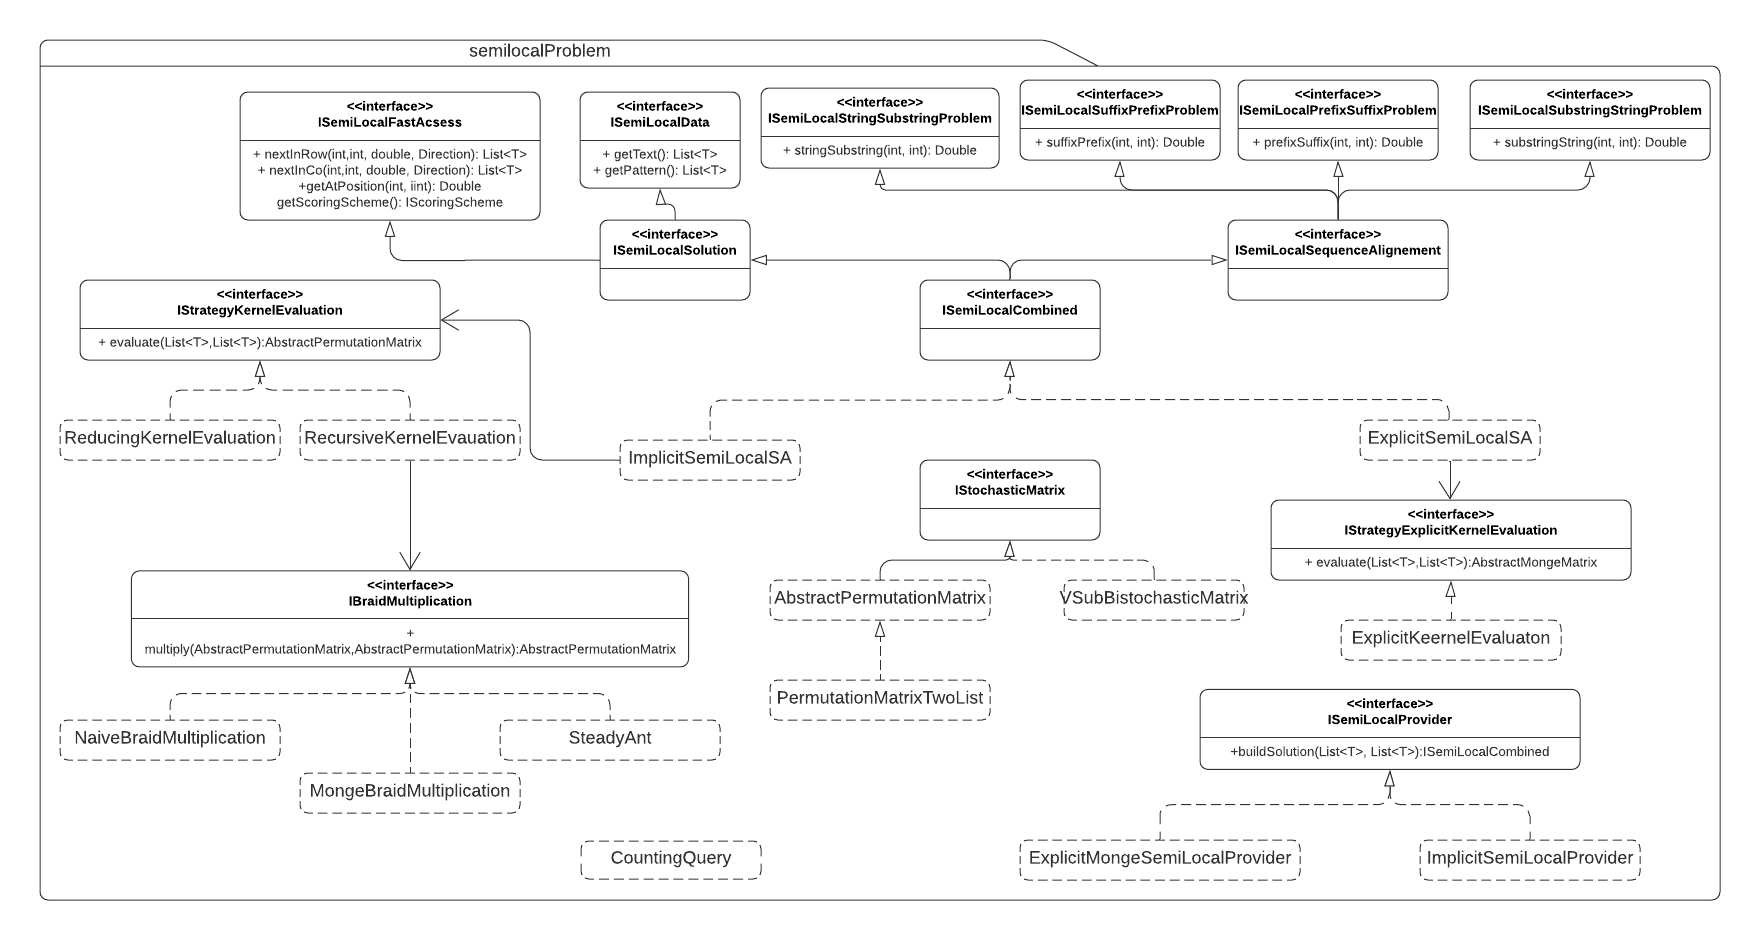
\includegraphics[height=0.72\columnwidth,angle=90]{figures/Library.png}
    \caption{Диаграмма классов UML части библиотеки, относящейся к различным задачам, основанным на  \emph{semi-local} задачах. Часть деталей и классов опущена.}\label{fig:libraryProblem}
\end{figure}

\emph{ExplicitSemiLocalSA} хранит матрицу $H_{a,b}$ в явном виде.
В данном случае нет экономии памяти, но доступ к произвольному элементу матрицы константный $O(1)$. 
Для решения задачи \emph{semi-local} используется алгоритм \emph{smawk}~\cite{aggarwal1987geometric}, отвечающий операции  $\otimes$.

% Стоит отметить, что недавние исследования~\cite{gawrychowski2020submatrix}, позволяют добиться 
% Нужно ли описать scorinSCheme



% \emph{ISemiLocalProvider}, \emph{ISemiLocalCombined} === паттерн фабричный метод
% набор классов и интерфейсов связанных с \emph{}
% Strategy --- стратегия




\subsubsection{Модуль semilocalApplication}
В данном модуле реализованы алгоритмы\footnote{Детальное описание алгоритмов и их доказательств находятся в ~\cite{tiskin2006all}}, для следующих задач:
\begin{enumerate}
    \item \emph{CompleteAMatch}
    \item \emph{Minimal-inclusive ThresholdAMatch}
    \item \emph{WindowAMatch}
    \item \emph{WindowSubstring}
    \item \emph{FragmentSubstring}
    \item \emph{BoundedLengthSmithWatermanAlignment}
\end{enumerate}

Первая задача относится к нахождению значения максимального выравнивания заданного шаблона $p$ и всех префиксов текста $t$ из всевозможных суффиксов из данного префикса:
\begin{equation}
    h[j] = \max _{i \in 0 ..j} sa(p,t[i,j]), j \in 0..|t|
\end{equation}

В рамках второй задачи ставится задача нахождения всех непересекающихся повторов шаблона $p$ в тексте $t$, чьи длины минимальны, а значение выравнивания выше заданного порога похожести $h$.

В третьей задаче необходимо найти все подстроки текста $t$ (уже могут пересекаться) длины $w$, чье выравнивание с шаблоном $p$ больше заданного порога похожести $h$.

Все эти три задачи сводятся к анализу \emph{подматрицы} задачи 
\emph{semi-local}, отвечающей \emph{srting-substring}.
И, соответственно, в зависимости от выбранного алгоритма решения задачи \emph{semi-local} асимптотика алгоритмов решения этих задач $O(n \times m \times \log n)$ и $O(v \times  m \times n)$.


\begin{figure}
    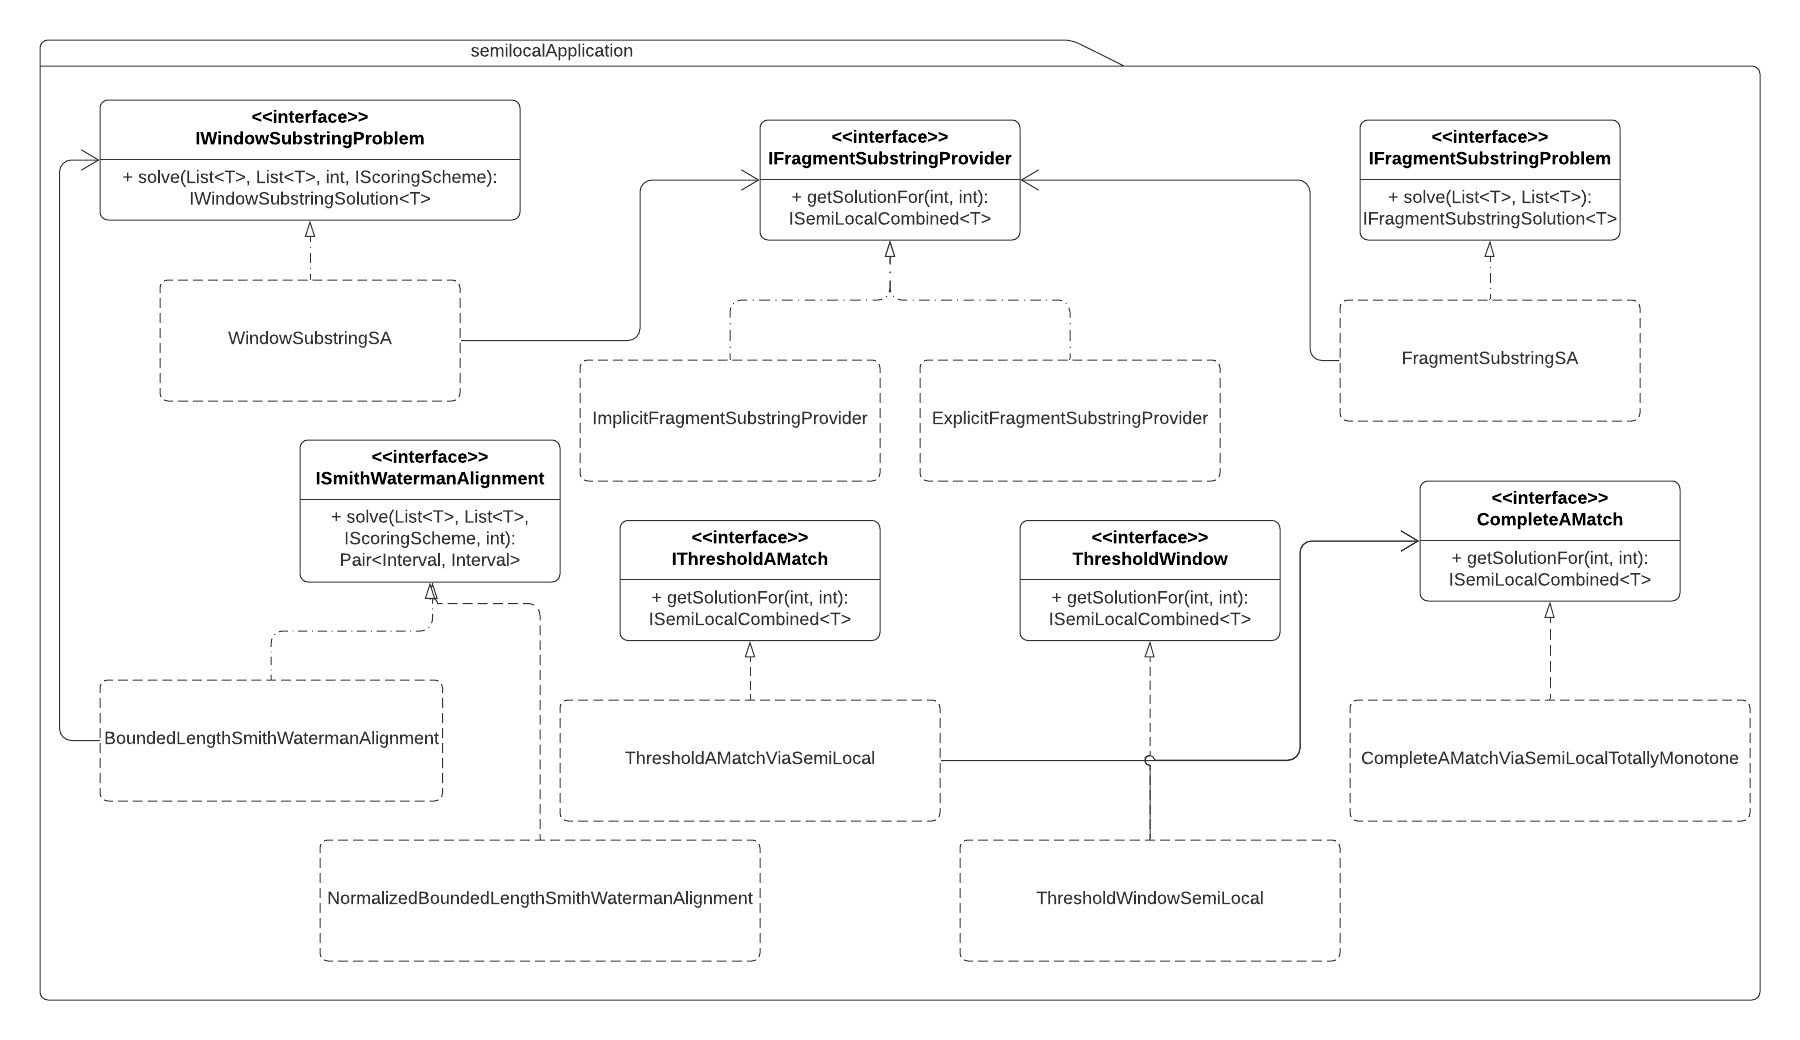
\includegraphics[width=\columnwidth]{figures/semiLocalApplication.png}
    \caption{Диаграмма классов UML части библиотеки, относящейся к \emph{semi-local} задачам. Часть деталей и классов опущена}\label{fig:libraryApplication}
\end{figure}


Задача \emph{FragmentSubstring} формулируется следующим образом: Для заданного множества интервалов (подстрок) $r$ из текста $t$ размера $m$ и текста $b$ размера $n$ необходимо вычислить \emph{semi-local} матрицу для каждого фрагмента из $r$ против $b$.
Имеет асимптотическую сложность $O(v^2 \times r \times  n \times \log m \times \log mv)$ \footnote{Существует возможность улучшить асиптотику до $O(v \times r \times  n \times \log^{2} m)$ } и $O(r \times n \times m  \times  log m)$.

Задача \emph{WindowSubstring}  является частным случаем   \emph{FragmentSubst-\\ring}, в которой размер фрагментов фиксирован.
Асимптотическая сложность решения уже будет $O(n \times m \times \log n)$ и $O(v^2 \times  m \times n)$.

Обе задачи основаны на двоичном разложении числа и предподсчете \emph{semi-local} решений, отвечающих данным разложениям.

Задача \emph{SmithWatermanAlignment} относится к локальному выравниванию.
В рамках данной задачи необходимо вычислить значение максимального локального выравнивания между $a$ и $b$, т.е найти пару подстрок, на которых достигается максимальное выравнивание.
Очень часто данная задача представляет интерес с различными ограничениями~\cite{arslan2004dynamic}.
Например, ограничения на минимальную длину подстрок.
Данное ограничение реализовано с помощью алгоритма из ~\cite{tiskin2019bounded} и инкапсулировано в соответствующем классе  \emph{BoundedLengthSmithWaterman-\\Alignment}.
Как отметил автор статьи, можно реализовать нормализованную версию данной задачи с применением \emph{BoundedLengthSmithWa-\\terman Alignment} к алгоритму из \cite{arslan2004dynamic}.

Нетрудно заметить, что часть алгоритмов в той или иной степени может быть адаптирована к задачам поиска повторов в документации.
Для задачи поиска по образцу такими кандидатами являются алгоритмы для решения задачи \emph{Minimal-inclusive ThresholdAMatch} и \emph{WindowSubstring}.
Для задачи поиска групп повторов могут быть применены  алгоритмы для \emph{WindowAMatch},
\emph{Minimal-inclusive ThresholdAMatch},\\\emph{BoundedLengthSmithWatermanAlignment} и \emph{semi-local}.

Адаптация алгоритмов к поиску повторов описана в следующем разделе.
Экспериментальная проверка асимптотики части алгоритмов, а так же их потенциальная возможность применения к большим данным даны в главе \ref{appob}.

% Соответствующая адаптация части алгоритмов описана в следующем разделе.
